

%\documentclass[conference]{IEEEtran}
\documentclass[12pt,a4paper]{article}
\usepackage{fullpage}

\usepackage{graphics}
\usepackage{color}
\usepackage[pdftex]{hyperref}
\usepackage{graphicx}
\usepackage{amssymb}

\begin{document}

\title{A Survey of Physical Design Techniques of Information Systems}


\author{Karim Ali and Sarah Nadi\\
\{karim, snadi\}@cs.uwaterloo.ca \\
David R. Cheriton School of Computer Science\\
University of Waterloo\\
}


% make the title area
\maketitle


\begin{abstract}
%\boldmath
The abstract goes here.
\end{abstract}

\section{Introduction}

Database users write queries and updates using a "user-friendly" language such as SQL without having to worry about how the underlying data is stored. Physical
database design is concerned with the actual storage of data on disk. This means how the files are organized, and how they are accessed. Data is stored in the
form of records in files which reside on a physical disk. In this sense, we try to find the most efficient way possible to store and access the data such that
queries are answered and executed efficiently. This is reflected in designing proper indexing techniques, partitioning data for more efficient access, designing
materialized views, data clustering, data compression, striping, mirroring and denormalization~\cite{lightstone2007physical}. 

This includes which indices to use, and in which order to access the tables~\cite{finkelstein1988physical} and so on.

This survey presents the different physical design patterns that have been used in different types of information systems. The systems discussed in this survey
are disk based relational databases, main memory relational databases, data warehouses, and XML databases. The aim of this survey is not to explain the details
of every data structure used in physical design, but rather to compare how the different data structures have been used in these systems. This includes
explaining how alterations or additions are made to data structures to fit the specific needs of every system. For a complete reference on the details of the
data structures used in physical database design, please see (CITE HERE). 


The rest of the survey is organized as follows. Section~\ref{SEC-ELEMENTS} first explains different elements of physical database design. For example, this
includes explaining what indexes are and briefly mentioning what the different types of indexes used in information systems are. After explaining the different
elements of physical database design, Section~\ref{SEC-DIFFSYS} discusses how each of the four systems uses these elements to improve its efficiency.
Sections~\ref{SEC-DDRDB},~\ref{SEC-MMDB},~\ref{SEC-WAREHOUSES},~\ref{SEC-XML} discuss Disk Based Databases, Main Memory Databases, Data Warehouses, and XML
Databases respectively. Throughout these sections, comparisons are made as to how the different elements have been modified to fit the needs of each system.
Section~\ref{SEC-AUTO} then presents physical database design can be automated. Section~\ref{SEC-OPEN} mentions some of the open problems of physical database
design, and suggests possible solutions. Finally Section~\ref{SEC-CONCL} summarizes and concludes this summary.



\section{Elements of Physical Database Design}
\label{SEC-ELEMENTS}

\subsection{Index Structures}

The first physical database design decision to be considered is the choice of indexes to be implemented. The concept of indices has been around for a long time.
Just like and index at the end of the book is provided to help find certain content faster, indices in an information system help find content in tables faster.
The main idea of an index is to have each record in a table have a unique identifier (primary key) and then organize these identifiers in a certain way that
allows for fast access of a specific record. Of course, indexing can be done on any column in the database and not necessarily the primary key. There are many
type of indexes that have been used in information systems.

B-trees (short for Balanced Trees) are the most used database index structure.  The B-tree is essentially similar to the traditional Binary Search Tree, but
instead of having one value per node, a B-tee can have many values per node~\cite{comer1979ubiquitous} as shown in Figure (PUT A FIGURE FOR A B TREE HERE).
B-trees are suitable for relational databases since the cost of retrieval in a B-tree is at most proportional to: $log_{d}\frac{n+1}{2}$. The cost of insertion
and deletion is at most proportional to $log_{d}n$ due to the possibility of progressing back up the tree to balance it after an insertion or a deletion.
Although B-trees do well in retrieval, deletion and insertion, they do not perform well in sequential search. 


Different variations of B-trees have been used. For example, $B^{+}-trees$ are now the main method of indexing in Disk Based Relational Databases (DRDB). These
will be discussed in Section~\ref{SEC-DDRDB}. The T Tree has been proposed for main memory databases, and will be discussed in Section~\ref{SEC-MMDB}. Cache
sensitive indexes were then proposed. A variation of T Trees, Cache Sensitive T-Trees (CST-Trees) was introduced, and is also discussed in
Section~\ref{SEC-MMDB}. On the same note, Cache Conscious $B^{+}-trees$ and Prefetching $J^{+}-Trees$ are also discussed in Section~\ref{SEC-MMDB}. 


Of course, there are other indexing techniques used such as hash tables, and bitmap indices. For example, Bitmap indices are commonly used in Data Warehouses,
and will be discussed in details in Section~\ref{SEC-WAREHOUSES}.


\subsection{Materialized Views}

In a large database system, there are usually a few complex queries that require the joining of many large tables. If these queries are frequently run, then the
database performance is likely to suffer, and users have to wait for a long time to get the results back. If we know these queries beforehand, it makes sense to
simply store the results of the queries on disk instead of recomputing them each time. Oracle 8i (SOURCE) introduced materialized views to fit this purpose. By
precalculating the
results of a complex query, and storing them in a table on disk, the new table with the results is very likely to be much smaller than the original tables
decreasing I/O access costs and thus increasing performance~\cite{lightstone2007physical, chaudhuri1998overview}. Once a materialized view exists, the user can
either explicitly query the materialized view, or enter the original query, and have the query optimizer rewrite the query to use the materialized views instead
of the original tables. Many query optimization techniques have relied on rewriting queries using views (E.g.~\cite{levy1995answering, gupta1995aggregate,
goldstein2001optimizing,
abiteboul1998complexity}), but discussing the details of the rewriting is beyond the scope of this survey.


Despite the fact that materialized views provide a significant improvement in performance, we cannot simply create a materialized view for each common query. To
begin with, materialized views consume disk storage which might be limited. The second, and main, problem with materialized views is their maintenance. Ensuring
that the views have the most up to date data is tricky, and may outset the benefit of using materialized views if it is not properly designed. Finally, having
several materialized views may increase the cost of searching for the appropriate view to use during the query optimization stage. Data warehouses heavily rely
on materialized views since they have many queries with several joins. This will be discussed in details in Section~\ref{SEC-WAREHOUSES}.



\subsection{Partitioning}

Partitioning is an important aspect of physical design as it reduces table scanning time. There are two main categories of partitioning: horizontal partitioning
and vertical partitioning. Horizontal partitioning divides the table into sets of table rows where each row or record still has all the attributes of the table.
For example, dividing the data by date where all data dating less than year 2000 lies in one partition while all data dating more lies in another. On the other
hand, vertical partitioning reduces the width of the dataset by storing some attributes in one table, and some in another.
The main advantage of any type of partitioning is to reduce the amount of time it takes to scan a table which in turn improves performance. For example, if a
table has 1000 records, and a query is only using the first 20 records then having these 20 records in a partition containing 50 records will save time as
opposed to examining all the 1000 records. Further classification in partitioning is single vs group horizontal or vertical
partitioning~\cite{gruenwald1990database}. Horizontal partitioning just divides the data into partitions where each group contains complete tuples. Group
horizontal partitioning groups tuples that are more frequently used together. Single vertical partitioning divides a relation into groups each of which contains
only one type of attribute. Group vertical partitioning divides the data vertically such that attributes that are commonly required together are physically
stored together.


\subsection{Clustering}
When only records satisfying certain criteria are need from a table, it is often unnecessary to scan the whole table. For example, if only records that occurred
in January 2010 are needed, then querying all the table would be an extremely unnecessary overhead. This is where clustering comes in. Clustering reflects how
the records are physically located together on disk. Records that are likely to be queried together will be stored physically together to avoid querying the
whole table. For the previously mentioned example, the data can be clustered by month, such that all the records of January 2010 are physically in the same
page, for example. In this case, only this page will need to be read. As
people realized the potential of clustering, multidimensional clustering was introduced where data is clustered based on different criteria at the same time.

\subsection{Other Physical Design Techniques}

There are other physical design methods to improve the performance of the information systems~\cite{lightstone2007physical}. For example, data compression can
be used to make more data fit into a fixed amount of disk space such that it can be access faster. Data striping is used to distribute data that is accessed
together across multiple disks. This allows the data to be retrieved faster through parallelism. Database reliability is also improved through mirorring which
involves duplicating the data on multiple disks. Finally, refining the global schema to reflect query and transaction requirements is also sometimes used. This
is called denormalization.

\section{Physical Design of Different Information Systems}
\label{SEC-DIFFSYS}

Given the different physical design methods explained in the previous section, we now look at how these methods apply to different types of information systems.
Mainly, how they apply to Disk-based relational database systems, main memory relational database systems, data warehouses, and XML databases. We mainly focus
on the first four techniques discussed in Section~\ref{SEC-ELEMENTS} as these are the main design decisions involved in physical design.


\subsection{Disk Based Relational Database System (DRDB)}
\label{SEC-DDRDB}

Relational Databases were first introduced by Codd~\cite{codd1970relational}. In relational databases, users specify the actions they want to execute without
having to worry about how these operations will actually be performed. This is where the role of physical design comes in. Physical design specifies the access
paths used to get data from the tables. 


\subsubsection{Index Structures}

There are many variations of B-trees. In relational databases, the most popular index is the $B^{+}-tree$. The $B^{+}-tree$ is a variant of the B  tree which is
becoming the main indexing method supported by many databases such as DB2, Oracle, and SQL Server~cite{lightstone2007physical}. The main difference between the
$B^{+}-trees$ and the B-tree is that only leaf nodes contain data pointers in a $B^{+}-tree$. (COMPARE COST HERE). In Prefix $B^{+}-trees$, instead of using the
actual key value of a record, a prefix from the key value is used to decrease the storage size needed which will in turn allow more records to be stored per
node thus decreasing the height of the tree.

The B+tree is the main indexing method used in current relational databases~\cite{lightstone2007physical}. B+trees have been successful in relational databases
since data is ultimately recorded in files. Since B+trees have a high fanout, they allow less I/O operations to access a specific data record which is stored in
a specific file.

MySQL mainly uses B Trees except for spatial data where the R Tree is used (http://dev.mysql.com/doc//refman/5.0/en/mysql-indexes.html)

\subsubsection{Paritioning}

MySQL only supports horizontal partitioning.

\subsection{Main Memory Relational Database System (MMDB)}
\label{SEC-MMDB}

A Main Memory Database (MMDB) (sometimes referred to as in-memory database) is one where the data resides in the main memory of the system rather than on a
disk~\cite{garcia1992main}. It should be noted that this is different from caching. Disk based database systems use the main memory to cache query results.
However, MMDB's primary copy of the data resides in main memory. MMDB have many implementation challenges that have been addressed throughout the research
community.


Garcia-Molina and Salem~\cite{garcia1992main} mention some of the challenges involved. One is concurrency control. In disk based databases, locks are tracked
through a hash table, but the actual objects on disk do not contain lock information. On the other hand, in MMDB, lock status is part of the object itself since
it is cheap to keep a number of bits for that. The next challenge is access methods. In disk-based databases, B-Trees are used to index the data for faster
access. B-Trees have a short bushy nature to try to decrease the height of the tree to decrease the number of I/O accesses. Since I/O access is not a problem in
MMDB, longer tree structures are used since its cheap to access main memory. Another point is that data values do not need to be stored in the index itself
since they will be stored in main memory anyways so there are no performance gains from storing them in the index itself. Table~\ref{tab:mmdbsumm} summarizes
the physical design elements of MMDBs.

\begin{table}[t!]
\centering
\scalebox{0.7}{
\begin{tabular}{p{3cm}|p{6cm}|p{6cm}}
\hline
 \textbf{Physical Design Element} & \textbf{Desired Features} & \textbf{Methods/Structures Used}\\
\hline\hline
Index Structures & \begin{itemize}
                    \item No need to store actual values in index \item Larger node size that is aligned with cache line size for cache consciousness
                   \end{itemize} & \begin{itemize}
                                    \item B Tree
\item B+ Tree
\item CSB+ Tree
\item pB+ Tree
\item T Tree
\item CST Tree
\item CSS Tree
                                   \end{itemize}\\
\hline
Materialized Views & \begin{itemize} \item Not needed since processing and memory access is cheap \end{itemize}& N/A\\
\hline
Partitioning & \begin{itemize} \item Only needed in secondary storage to speed up reloading in case of a crash \end{itemize} & \begin{itemize}
                                                                                            \item Horizontal Partitioning
\item Single Vertical Partitioning
                                                                                           \end{itemize}\\
\hline
Clustering & \begin{itemize} \item Not needed since sequential random or dispersed main memory access is not more expensive than sequential access \end{itemize}
& N/A

\end{tabular}
}
\caption{Summary of physical design of Main Memory Databases (MMDB)}
\label{tab:mmdbsumm}
\end{table}


\subsubsection{Index Structures}

Two considerations are taken when designing index structures for MMDB. The first is that the data resides in main memory and not on disk, and so many of the
considerations taken for I/O operations is no longer there. Instead of focusing on disk access and disk storage, the data structures for main memory
databases should focus on the efficient use of CPU cycles and memory~\cite{lehman1986study}. The second is having index structures cache conscious. Cache
memories improve performance by holding recently referenced data~\cite{smith1982cache}. If the memory reference is found in the cache, then execution proceeds
at processor speed. Otherwise, the data has to be fetched from main memory. With the big difference between processor speed and main memory speed, cache misses
are still relatively expensive. Lots of research work has shown that cache performance is very critical in MMDBs~\cite{boncz1999database,rao1999cache}. This is
because the big difference between processor speed and main memory access speed. Thus, a cache miss is still relatively expensive in main memory databases.
Accordingly, we will see that many of the index data structures proposed for main memory databases focused on being cache conscious or cache sensitive. In
summary, a main memory index should be able to reduce overall computation time while using as little memory as possible~\cite{lehman1986study}. It should also
be noted that unlike disk based systems where it is advantageous to store actual attribute values in the index, main memory systems do not require that.
Instead, pointers to the actual attribute values can be used. This, in turn, will reduce the size of the index which is preferable in this case.

In this section, we talk about three families of index structures used in MMDB: B Trees, T Trees, and Binary Search Trees. There are more recent index
structures developed for MMDB such as J+ Trees~\cite{luan2009prefetching}, but which have not gained much popularity, and so we do not discuss them in our
survey. Table~\ref{tab:mmdbindexsumm} summarizes the features of the different index structures discussed in this section with respect to MMDB. The T Tree is
the most used index for MMDB (E.g. MySQL CLuster). However, there are other indexes used as well. For example, IBM's solidDB uses Trie (or prefix tree) for its
indexing. For their purposes, it served as a good index for main memory since it eliminates the need for many key comparisons~\cite{ibmsoliddb}.


\begin{table}[t!]
\centering
\scalebox{0.7}{
\begin{tabular}{p{2cm}|p{6cm}|p{6cm}}
\hline
 \textbf{Index Structure} & \textbf{Features suitable for MMDB} & \textbf{Cache Consciousness}\\
\hline\hline
B Trees &
\begin{itemize}\item Good storage utilization
\item Reasonably quick searching
\item Fast updating
\end{itemize} 
& \begin{itemize}\item Reasonable cache behavior if node fits in cache line\end{itemize}\\
\hline
B+ Trees & 
\begin{itemize}
\item Wastes space since all data is stored in the leaves
\item Reasonably quick searching
\item Fast updating
\end{itemize} &
\begin{itemize}
\item Reasonable cache behavior if node fits in cache line\end{itemize}\\
\hline
CSB+ Trees & \begin{itemize}
              \item Same features of B+ Trees
             \end{itemize} &
\begin{itemize}
 \item Good cache performance due to improved locality \& lower tree height
\end{itemize}\\
\hline

pB+ Trees & \begin{itemize}
              \item Same features of B+ Trees
             \end{itemize} &
\begin{itemize}
 \item Improves cache miss performance by prefetching more data in each cache miss
\item Node size is also increased leading to the same benefits of CSB+ Trees
\end{itemize}\\
\hline
T Tree &  \begin{itemize}
              \item Contain pointers to data values instead of the values themselves leading to better space utilization
\item Node size is bigger leading to previous mentioned advantages
             \end{itemize} &
\begin{itemize}
 \item Cache behavior was not considered at time of design
\end{itemize}\\
\hline
CST & \begin{itemize}
       \item Binary search tree for maximum value of each node leads to faster search
\item More space efficient by removing pointers \& using array storage. Index calculation used to allocate values
      \end{itemize} &
\begin{itemize}
 \item Node size is aligned with cache line size to avoid misses
\end{itemize}\\
\hline
CSS Trees &  \begin{itemize}
       \item Fast traversal in $log_{m+1}n$ ($m$ is the number of keys per node)
\item Mainly suitable for read environments
      \end{itemize} &
\begin{itemize}
 \item Good cache behavior since $m$ is chosen to fit in the cache line size
\end{itemize}\\

\end{tabular}
}
\caption{Summary of index structures for Main Memory Databases (MMDB)}
\label{tab:mmdbindexsumm}
\end{table}


%cite~\cite{dewitt1984implementation}.

\subsubsection*{B Trees}
Although B Trees, explained in the previous section, are originally designed for disk based database systems, they were found to also be useful in
MMDB~\cite{lehman1986study}. In disk based systems, the B+ Tree is more used than the regular B Tree. However, in main memory databases, the B Tree would be
more suitable from a storage perspective since there is no gain from keeping all the data in the leaves. In a main memory system, this
would only waste space without improving performance. On the other hand, the B+ Tree uses multiple keys to search within a node. This means that
if the node fits in a cache line, this cache load can satisfy more than more comparison leading to better cache utilization~\cite{rao1999cache}. Therefore, B+
Trees in general have reasonable cache behavior.

However, the cache behavior of B+ Trees could still be improved. Therefore, Rao and Ross~\cite{rao2000making} propose Cache Sensitive B+-Trees
($CSB^{+}-Trees$)~\cite{rao2000making} as an index structure for main memory. To do so, they eliminated most of the child pointers and had more keys in each
node to improve locality and reduce tree height~\cite{luan2009prefetching}. Since the number of cache misses in search operations is proportional to the height
of the tree, $CSB^{+}-trees$ have fewer cache misses, and thus better performance.

Chen et al.~\cite{chen2001improving} propose using prefetching to improve the performance of B+ Trees. They call the new index structure prefetching B+ Tree
(pB+ Tree). Since current computer systems can prefetch different data simultaneously, the authors take advantage of this. The idea here is to increase the node
size of B+ Trees and employ prefectching at the same time. In a B+ Tree, every time we move down a level in the tree, a cache miss occurs. Accordingly,
prefetching larger sizes nodes means that we can overlap multiple cache misses before they occur. This is because in one cache miss, extra data is retrieved in
parallel with the originally requested data if it can be predicted sufficiently early. Figure~\ref{fig:prefetching} shows how prefetching retrieves the same
data in less time. This method, however, does not eliminate the full cache miss latency with every level in the tree.

\begin{figure}[!t]
\centering
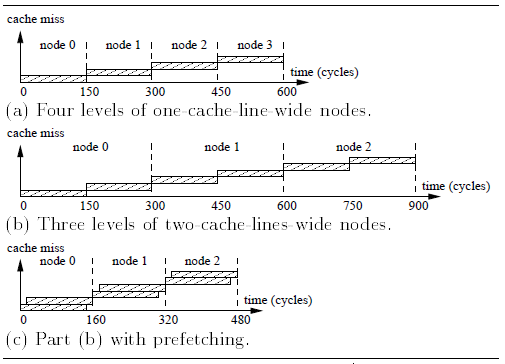
\includegraphics[width=7cm]{figs/prefetching.png}
\caption{Performance of various B+ Tree searches where a cache miss to memory takes 150 cycles and a subsequent access can begin 10 cycles
later~\cite{chen2001improving}}
\label{fig:prefetching}
\end{figure}

\subsubsection*{T Trees}
Lehmen and Carey~\cite{lehman1986study} introduce a new index structure, the T Tree, which combines the features from AVL Trees and B Trees that are suited to
main memory. Figure~\ref{fig:ttree} shows the proposed structure of the T Tree. They run some experiments on data residing in main memory to compare the
performance of the T
Tree to existing structures. All structures were modified to contain pointers to data values rather than the data values themselves. The structures
compared included  AVL Trees, simple arrays, B Trees, Chained Bucket Hashing, Extendible Hashing, Linear Hashing and Modified Linear Hashing. Their
experiments showed that for unordered data, Modified Linear Hashing gave the best performance, and for ordered data, T Trees gave the best performance for a mix
of searches, inserts and deletes. This is mainly because a T node contains many elements which results in good update and storage characteristics. The T Tree
was the first index structure specifically designed for main memory databases.

Although T Trees have been specifically designed for MMDB, they did not consider the cache behavior at that time~\cite{rao1999cache}. Although many keys are
fit into one node, only the two end keys are used for comparison leading to low node utilization. Similarly, array binary search trees have the same problem. 

\begin{figure}[!t]
\centering
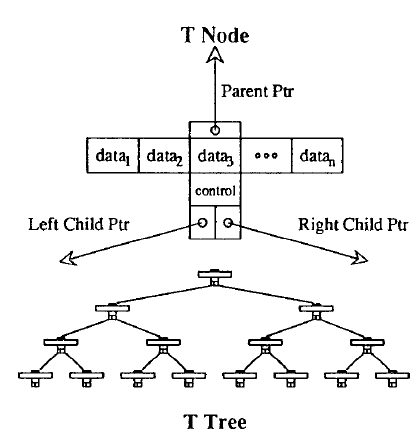
\includegraphics[width=7cm]{figs/Ttree.png}
\caption{T Tree by Lehmen and Carey~\cite{lehman1986study}}
\label{fig:ttree}
\end{figure}

T Trees were the main index structure used for main memory databases for some time after their proposal. However, it was discovered that B+-trees outperform
T-Trees on modern processors because of the growth of cache miss latency relative to processor speed~\cite{rao1999cache,lee2007cst}. This is because the height
of the tree is high which makes the total number of memory accesses from the root to the leaf node higher. The other reason is that the node size is not aligned
with the cache line size. Another problem with T-Trees is that there is a big waste of space in the cache because unnecessary data is brought into the cache.
Additionally, record pointers stored in the tree take up a lot of space.

To resolve these issues, Lee et al.~\cite{lee2007cst} propose the Cache Sensitive T-Trees (CST-Trees). This is achieved in the following ways. First, a binary
search tree whose node values are the maximum key of each node in the T Tree is constructed. That way, for a given value, the node containing this value could
be quickly located through searching the binary tree. Second, the need to store pointers is eliminated by storing the tree in an array and locating the
necessary nodes through index calculation. Finally, node sizes are aligned with cache line size such that there are no cache misses when accessing data in each
binary search tree in the array.

\subsubsection*{Cache Sensitive Search Trees (CSS-Trees)}

Binary Search Trees have poor cache behavior when the array is much bigger than the cache. Rao and Ross~\cite{rao1999cache} propose the Cache Sensitive Search
Tree (CSS-Tree) to improve this cache behavior. To do that, the search tree is stored as a directory in an array. The number of keys per node is chosen such
that the whole node fits in a cache line. This improves local searching within a node to just one cache miss. They also hard-code the traversal within a node
such that finding the next node happens in $log_{m+1}n$ times rather than $log_{2}n$ times in a binary search tree where $m$ is the number of keys per node.
However, CSS Trees are only suitable for read environments since they eliminate nearly all child pointers, thus removing the support for incremental update.

\subsubsection{Materialized Views}
From our literature survey, it seems that materialized views are not used in MMDB. This makes sense since the problems materialized views try to address are
not present in MMDB. That is, the cost of computing complicated join queries is much less in MMDB due to the low cost of accessing the data in memory.
Accordingly, the maintenance cost of materialized views in MMDB will outweigh their minimal benefit.

\subsubsection{Partitioning}

Partitioning is used in disk based systems to divide the data into the physical pages in a way that will yield the best performance. This could be through
vertical partitioning or horizontal partitioning, as previously explained. In main memory databases, we do not have the issue of expensive disk access which
makes partitioning in memory unnecessary as it will not save any costs. However, partitioning is needed in the secondary storage of the data on
disk~\cite{gruenwald1990database}. Disk storage is still used as a backup of main memory databases. When a crash occurs, a reload of the database from disk or
archive memory takes place. In order to avoid page faults caused by referencing data that is still being reloaded, the reloading process must be designed to be
efficient in loading the important data such that the database users are not affected. An efficient MMDB reload takes into consideration the number of I/Os for
reload and the number of main memory references during transaction processing. Gruenwald and Eich~\cite{gruenwald1990database,gruenwald1990choosing} show that
horizontal partitioning is the most suitable when the database performs more modifications than tuple deletions and more selections that projections and joins.
Single vertical partitioning is chosen in the other cases. They also show that if we just concentrate on the reload performance (i.e the number of I/Os for
reload), then single vertical partitioning is always the best choice.


\subsubsection{Clustering}
Clustering in disk based systems is important because sequential I/O access is cheaper than random or dispersed I/O access. This is not the case with main
memory, and so clustering is not needed in MMDB~\cite{garcia1992main, moldovan2008databases}. Therefore, components of one object may be spread across memory
without impacting performance.



\subsection{Data Warehouses}
\label{SEC-WAREHOUSES}
A data warehouse is a subject-oriented, integrated, time-variant, and non-volatile collection of data and decision support technologies, aimed at enabling the knowledge worker (executive, manager, analyst) to make better and faster decisions \cite{560407, 248616}. More than half of IT executives named Data warehousing as the highest-priority post-millennium project for them \cite{sen2005comparison}. The value of data warehousing for an organization depends on the organization's need for reliable, consolidated, unique and integrated reporting and analysis of its data, at different levels of aggregation.

Data warehousing has been shown useful in many industries: manufacturing (for order shipment and customer support), retail (for user profiling and inventory
management), financial services (for claims analysis, risk analysis, credit card analysis, and fraud detection), transportation (for fleet management),
telecommunications (for call analysis and fraud detection), utilities (for power usage analysis), and healthcare (for outcomes analysis) \cite{248616}.

Data warehouses tend to be extremely large, in fact it is quite possible for a data warehouse to store tens of petabytes of data while loading tens of terabytes of data everyday \cite{thusoo2010data}. Datta et al. \cite {628286} notes that the information in a data warehouse is usually multidimensional in nature, requiring the capability to view the data from a variety of perspectives. Aggregated and summarized data become more crucial than detailed records in such environment. Therefore, the workloads are query intensive with mostly ad hoc, complex queries, often requiring computationally expensive operations such as scans, joins, and aggregation. Performing such operations on large amounts of data, like in the case of data warehousing, complicates the situation further. Moreover, the results have to be delivered interactively to the business analyst using the system.

Although data in a data warehouse is extracted and loaded from multiple on-line transaction processing (OLTP) data sources (including DB2, Oracle, IMS databases, and flat files) using Extract, Transfer, and Load (ETL) tools (see Figure \ref{fig:dw}), a data warehouse is usually maintained seperately from the organization's operational databases \cite{sen2005comparison, 248616}. This architecture can be justified owing to the fact that operational databases are finely tuned to satisfy known OLTP requirements and functionalities which are quite different from that of on-line analytical processing (OLAP) which is supported by data warehousing. Analyzing data for decision support usually requires consolidating data from many heterogeneous sources of varying quality, or use inconsistent representations, codes and formats. Moreover, understanding trends or making predictions requires historical data, whereas operational databases store only current data. In OLAP, there's a need to support multidimensional data models and operations which requires special data organization, access methods, and implementation methods, not generally provided by DBMSs targeted for OLTP \cite{248616}. Finally, in data warehousing, query throughput and response times are more important than transaction throughput which is the major performance metric for operational databases.

\begin{figure}[!t]
\centering
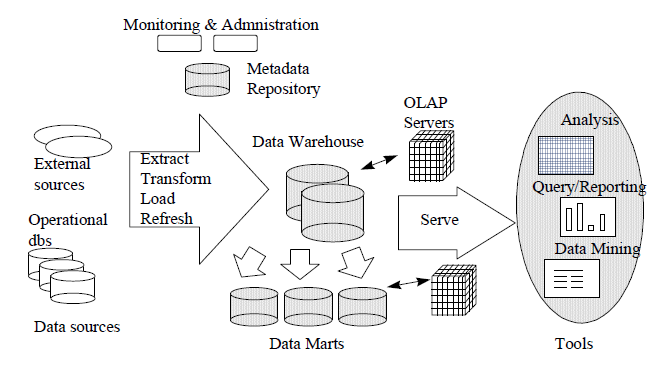
\includegraphics[width=9cm]{figs/dw.png}
\caption{Data Warehousing Architecture \cite{248616}}
\label{fig:dw}
\end{figure}


\cite{Cheung20011}
ROLAP
          o Data is stored in relational databases.
          o support for multi-dimensional view of data is achieved thru star scheme
          o Support extensions to SQL.
          o Efficiently implement the multidimensional data model and operations.
          o Ex: Microstrategy.
MOLAP
          o Directly store multidimensional data in special data structures (arrays).
          o Implement the OLAP operations over these special data structures.
          o Snowflake Schema. \cite{kimball2009data}
          o Fact Constellations.
          o Ex: Essbase (Arbor), statistical DBMSes.

hierarchical data clusters \cite{karayannidis2008hierarchical}

star schema
fact table

Typical Operations
    * Data Cleaning
    * Load
    * Refresh

Joins in data warehouses are usually expensive since the fact table (the largest one) participates in every join \cite{628286}

\subsubsection{Index Structures}
\paragraph{Tree-based Indexes}
B-tree (B+ trees but commonly referred to as B-trees) \cite{253268}, R-tree \cite{602266, Cheung20011}, K-D-B-tree \cite{582321}, BV-tree \cite{223796}, UB-tree
\cite{bayer1997universal}


\paragraph{Bitmapped Join Indexes}
\cite{212001}


\paragraph{Projection Indexes}
Involves positional indexing where tuples are accessed based on their ordinal position \cite{628286}

\paragraph{Bit-sliced Indexes}


\subsubsection{Partitioning}
\cite{thusoo2010data}
\paragraph{Vertical Partitioning}

\paragraph{Horizontal Partitioning}

\subsubsection{Materialized Views}
not very useful since most queries are ad-hoc \cite{653447}
\cite{355309}

\subsection{XML Databases}
\label{SEC-XML}

XML (eXtensible Markup Language) is increasingly being used as a data exchange format. Accordingly, the ability to store and manage XML documents is needed.
Salminen and Tompa~\cite{salminen2001requirements} define an XML database as ``a collection of XML documents and their parts, maintained by a system
having capabilities to manage and control the collection itself and the information represented by that collection.'' Salminena and Tompa also highlight some of
the requirements of an XML database system. These requirements include dealing with namespaces, Internet resources, querying parts of an XML document, and
transformations of XML documents.

There are two ways in which an XML database system can be designed. The first is to have the database internally translate the XML document into relational
tables (XML-enabled databases). The second is to have data structures that can persistently store XML documents (native XML databases). In this section, we will
discuss how the database's physical design needs to be adapted in both cases. Other challenges such as expressing and executing queries and updates are faced in
XML database design, but these are beyond the scope of this survey.


%eXist~\cite{meier2009exist} and TIMBER~\cite{jagadish2002timber} are two of the famous research efforts to design a native XML database.

\subsubsection{Index Structures}

Despite the special nature of XML documents, the same index structures used in relational databases can still be utilized in XML databases. However, some
adjustments may need to be made to fit the nature of the XML documents. For XML-enabled databases, XML documents are usually represented as relational tables,
and then indexed similar to other tables. Pal et al.~\cite{pal2004indexing} describe how this is done in Microsoft SQL Server 2005. To start with, a new data
type called `XML' was introduced. This data type could contain values of complete XML documents, or just fragments of XML data. First, the different nodes in
the XML data are labelled with the ORDPATH~\cite{o2004ordpaths} mechanism. The XML data is then shredded into a relational table with five main columns:ORDPATH,
TAG, NODE\_TYPE, VALUE, and PATH\_ID. This information is then stored in a $B^{+}-tree$ as the primary index of the XML type. Additionally, a secondary index
can be created on any of the columns of the primary index to speed things up.


For native XML databases such as eXist~\cite{meier2009exist} or TIMBER~\cite{jagadish2002timber}, $B^{+}-trees$ were still used to index the XML documents.
However, in contrast to XML-enabled databases, the XML data is not first stripped into a relational table. eXist uses a number schema to assign unique
identifiers to each node in the XML document. These unique number identifiers allow the determination of any node's parent, sibling or possible child nodes.
Four index files are created for XML data where all the indexes are based on $B^{+}-trees$. One index manages the collection hierarchy, one index collects nodes
in a paged file and associates unique node identifiers to the actual nodes, one index indexes elements and attributes, and the last index keeps track of word
occurrences and is used by the fulltext search extensions. Oracle uses a similar technique for indexing its XML content where an XMLIndex table is created for
XML entries~\cite{oracleXML}. This table contains a unique identifier for the XPath leading to the node, the row id of the table used to store the XML data,an
order key that identifies the hierarchal positioning of the node, a locator key used for fragment extraction, and the text value of the node.

TIMBER also uses a similar numbering schema. There are minor differences between the two numbering techniques, but the main idea is the same. The numbering is
based on three values of a node: its start label, its end label, and its level (i.e. nested depth). On the other hand, Sedna~\cite{taranov2010sedna} uses a
different reasoning to produce its numbering schema. Sedna assignes string identifiers to nodes such that they are lexically ordered according to the position
of the node. Despite the differences in the ways the numbering is constructed, it seems that that no novel indexing structure is needed for XML databases. The
problem is rather how to assign the nodes unique identifiers (the numbers or labels in the numbering schema) that can be used as identifiers in the index to
reflect the XML document structure.


Besides indexing the actual nodes, path indexing is also common in XML databases since usually queries search for a specific path. This is done by clustering
together all the IDs of nodes on a given path, and creating an index for them~\cite{milo1999index, arion2008path}.

\subsubsection{Materialized Views}

The main idea behind using materialized views is to rewrite queries using these views so that they run more efficiently. This is very important in XML
Databases since XQuery and XPath queries are complicated~\cite{arion2007structured}. The semi-structured nature of
XML data, and the expressiveness of most XML querying languages, view selection for optimization becomes a more complicated
problem~\cite{tang2009materialized}. Therefore, the choice of which views to materialize becomes more complicated in XML database. Much work has been
done on rewriting XML queries using views~\cite{arion2007structured, balmin2004framework, aouiche2006clustering, tang2008multiple}. However, this problem is not
within the scope this survey.

\subsubsection{Partitioning}
In XML-enabled databases, inlining during the shredding of the data such that children nodes that occur only once are stored with the parent node produces
better partitioned data~\cite{tatarinov2002storing}. Inlining shreds a document into sets of tables according to the document schema which leads to better
performance because queries tend to access less data. Such inlining is similar to horizontal partitioning~\cite{ramanath2003searching}. Additionally, it is
common to horizontally partition the mapped relational tables such that nodes of the same type are stored together~\cite{amer2002overview}.

\subsubsection{Clustering}
Clustering in XML databases follows the heuristic that sub-elements are likely to be queries with an element~\cite{jagadish2002timber}. Accordingly, elements
and their subelements are clustered together. In general, storing the XML data in document order it thought to be the best technique for efficient querying.
Additionally, Lian et al.~\cite{lian2004efficient} suggest clustering XML documents by structural similarity to produce more efficient access. This is done by
representing the documents as a structure graph (s-graph), and then identifying clusters based on similarity using a clustering algorithm.
Nayak~\cite{nayak2008fast} also proposes a similar clustering mechanism for XML data. Her technique is also based on structural similarity, but it is more
focused on the level structure of the XML documents.

\section{Real Databases (incorporate in previous section)}

Oracle Database uses B tree indexes and their subtypes such as Index-organized tables, reverse key indexes, descending indexes, B-tree cluster indexes. It also
uses Bitmap and bitmap join indexes, function based indexes and domain based indexes.


MySQL mostly uses B trees, except for spatial data where R trees are used and hash indexes are used for memory tables.

\section{Automating Physical Database Design}
\label{SEC-AUTO}

\section{Open Problems in Physical Database Design}
\label{SEC-OPEN}

Indexing in the cloud~\cite{wang2010indexing}.

Two-Tier Storage DBMS (using disk based and main memory dbs)~\cite{eo2008two}.

\section{Conclusions}
\label{SEC-CONCL}

%\bibliographystyle{IEEEtran}

\bibliographystyle{plain}
\bibliography{references}





% that's all folks
\end{document}


